\documentclass[a4paper]{article}
\usepackage{enumitem, amsmath, gensymb, graphicx, caption, amssymb, geometry, fancyhdr, arydshln, adjustbox}

\geometry{left=1in, right=1in, top=1in, bottom=1in}
\pagestyle{fancy}

\newcommand{\myName}{\textbf{Shantanu Ghodgaonkar}\\\textit{Univ ID}: N11344563\\\textit{Net ID}: sng8399\\\textit{Ph.No.}: +1 (929) 922-0614}
\newlist{qalist}{description}{1}
\setlist[qalist]{style=unboxed,leftmargin=0.5cm,labelwidth=2.5cm}


\title{Homework 2 Answers : ROB-GY 6003}
\author{\myName}
\date{\today}

\fancyhead{} % Clear existing header settings 
\fancyhead[L]{\today}
\fancyhead[R]{N11344563}


\begin{document}
	
	\begin{titlepage}
	    \centering
	    \vspace{2cm}
	    \Huge\textbf{Mathematics for Robotics \\ ROB-GY 6103 \\ Homework 3 Answers}
	    \vspace{1cm}
	    \\ \Large \today
	    \vfill
	    \Large \myName
	\end{titlepage}
	
	\begin{qalist}			
		\item[Question: 1.] \setcounter{equation}{0} %Nagy, Page 117, Prob. 4.1.5
%		Given two finite subsets ${\mathcal{S}}_{1}$ and ${\mathcal{S}}_{2}$ in a vector space $\mathcal{V}$ show that \[Span({\mathcal{S}}_{1} \cup {\mathcal{S}}_{2}) = Span({\mathcal{S}}_{1}) + Span({\mathcal{S}}_{2})\]
		\item[Answer:] 
%			Given, 
%			Two finite subsets ${S}_{1}$, ${S}_{2}$ in a vector space $V$ having Span
%			\begin{equation}
%				Span\{{S}_{1}\} = \{{x}_{1} \in \mathcal{X}|\exists n \geq 1 , {\alpha}_{1}, \ldots, {\alpha}_{n} \in \mathcal{F}, {v}^{1}_{1}, \ldots, {v}^{n}_{1} \in {S}_{1}, s.t. \; {x}_{1} = {\alpha}_{1}\cdot{v}^{1}_{1} + {\alpha}_{2}\cdot{v}^{2}_{1} + \ldots + {\alpha}_{n}\cdot{v}^{n}_{1}\}
%			\end{equation}
%			\begin{equation}
%				Span\{{S}_{2}\} = \{{x}_{2} \in \mathcal{X}|\exists m \geq 1 , {\beta}_{1}, \ldots, {\beta}_{m} \in \mathcal{F}, {v}^{1}_{2}, \ldots, {v}^{m}_{2} \in {S}_{2}, s.t. \; {x}_{2} = {\beta}_{1}\cdot{v}^{1}_{2} + {\beta}_{2}\cdot{v}^{2}_{2} + \ldots + {\beta}_{m}\cdot{v}^{m}_{2}\}
%			\end{equation}
%			
%			Combining subspaces ${S}_{1}$ and ${S}_{2}$ $i.e.$ combining ${Eq}^{n}(1)$ and ${Eq}^{n}(2)$, we get, 
%			\begin{equation}
%				\begin{aligned}
%					Span\{{S}_{1} \cup {S}_{2}\} = 
%					\bigl\{{x}_{1}+{x}_{2} \in \mathcal{X} \; |\;\exists \; n,m \geq 1 , {\alpha}_{1}, \ldots, {\alpha}_{n} \in \mathcal{F}, {\beta}_{1}, \ldots, {\beta}_{m} \in \mathcal{F},  \\
%					{v}^{1}_{1}, \ldots, {v}^{n}_{1} \in {S}_{1}, {v}^{1}_{2}, \ldots, {v}^{m}_{2} \in {S}_{2} \\
%					 s.t. \; {x}_{1} + {x}_{2} = ({\alpha}_{1}\cdot{v}^{1}_{1} + {\beta}_{1}\cdot{v}^{1}_{2}) +  \\
%					 ({\alpha}_{2}\cdot{v}^{2}_{1} +  {\beta}_{2}\cdot{v}^{2}_{2}) \\
%					 \cdot  \\
%					 \cdot \\
%					 \cdot  \\
%					 ({\alpha}_{n}\cdot{v}^{n}_{1} + {\beta}_{m}\cdot{v}^{m}_{2})\bigr\}
%				\end{aligned}
%			\end{equation} 
%			So, from ${Eq}^{n}(3)$, we get, 
%			\begin{equation}
%				{x}_{1} + {x}_{2} = ({\alpha}_{1}\cdot{v}^{1}_{1} + {\beta}_{1}\cdot{v}^{1}_{2}) +\\
%				 ({\alpha}_{2}\cdot{v}^{2}_{1} +  {\beta}_{2}\cdot{v}^{2}_{2}) \\
%				 \cdot\\
%				 \cdot\\
%				 \cdot\\
%				 ({\alpha}_{n}\cdot{v}^{n}_{1} + {\beta}_{m}\cdot{v}^{m}_{2})
%			\end{equation}
%			\begin{equation}
%				= ({\alpha}_{1}\cdot{v}^{1}_{1} + {\alpha}_{2}\cdot{v}^{2}_{1} + \ldots  + {\alpha}_{n}\cdot{v}^{n}_{1}) +
%				 ( {\beta}_{1}\cdot{v}^{1}_{2} +  {\beta}_{2}\cdot{v}^{2}_{2} + \ldots + {\beta}_{m}\cdot{v}^{m}_{2})
%			\end{equation}			
%			
%			Upon observation, we can deduce that  ${Eq}^{n}(5)$ =  ${Eq}^{n}(1)$ +  ${Eq}^{n}(2)$, i.e,
%			\begin{equation}
%				Span({S}_{1} \cup {S}_{2}) = Span\{{S}_{1}\} + Span\{{S}_{2}\}
%			\end{equation}
%			
%			\textbf{Q.E.D.}
%			
%		\item[Question: 2.(a)] \setcounter{equation}{0} %Nagy, Page 121, Prob. 4.2.1 (a)
%		\item[Answer:] Given set,
%			\begin{equation}
%				\left\{ \left[\begin{matrix}1 \\ 2 \\ 3\end{matrix}\right], 
%					\left[\begin{matrix}2 \\ 1 \\ 0\end{matrix}\right], 
%					\left[\begin{matrix}1 \\ 5 \\ 9\end{matrix}\right]
%				\right\}
%			\end{equation}
%			
%			To check for Linear Dependance,
%			\begin{equation}
%				{\alpha}_{1}\cdot\left[\begin{matrix}1 \\ 2 \\ 3\end{matrix}\right] + 
%				{\alpha}_{2}\cdot\left[\begin{matrix}1 \\ 1 \\ 0\end{matrix}\right] + 
%				{\alpha}_{3}\cdot\left[\begin{matrix}1 \\ 5 \\ 9\end{matrix}\right]
%				 = 0
%			\end{equation}
%			This gives us three equations, 
%			\begin{align}
%				{\alpha}_{1} + 2{\alpha}_{2} + {\alpha}_{3}= 0 \\
%				2{\alpha}_{1} + {\alpha}_{2} + 5{\alpha}_{3}= 0 \\
%				3{\alpha}_{1} + 9{\alpha}_{3}= 0
%			\end{align}
%			Substituting ${\alpha}_{1} = -3$, ${\alpha}_{2} = 1$ and ${\alpha}_{3} = 1$ in above ${Eq}^{n} (3), (4) \& (5)$
%			\begin{align}
%				{Eq}^{n} (3) \Rightarrow -3 + 2 + 1 = 0 \\
%				{Eq}^{n} (4) \Rightarrow -6 + 1 + 5 = 0 \\
%				{Eq}^{n} (5) \Rightarrow -9 + 9 = 0
%			\end{align}
%			$\therefore$ the given set is \textit{Linearly Dependent}. 
%			
%			So, we can express each vector as a linear combination of the remaining vectors of the set.
%			For example, 
%			\begin{equation}
%				\left[\begin{matrix}1 \\ 2 \\ 3\end{matrix}\right] = 
%				\frac{1}{3}\left[\begin{matrix}2 \\ 1 \\ 0\end{matrix}\right] +
%				\frac{1}{3}\left[\begin{matrix}1 \\ 5 \\ 9\end{matrix}\right]
%			\end{equation}
%			
%			\pagebreak
%			
%		\item[Question: 2.(b)] \setcounter{equation}{0} %Nagy, Page 121, Prob. 4.2.1 (b)
%		\item[Answer:] Given set,
%			\begin{equation}
%				\left\{ \left[\begin{matrix}1 \\ 2 \\ 3\end{matrix}\right], 
%					\left[\begin{matrix}0 \\ 4 \\ 5\end{matrix}\right], 
%					\left[\begin{matrix}0 \\ 0 \\ 6\end{matrix}\right],
%					\left[\begin{matrix}1 \\ 1 \\ 1\end{matrix}\right]
%				\right\}
%			\end{equation}
%			
%			To check for Linear Dependance,
%			\begin{equation}
%				{\alpha}_{1}\cdot\left[\begin{matrix}1 \\ 2 \\ 3\end{matrix}\right] + 
%				{\alpha}_{2}\cdot\left[\begin{matrix}0 \\ 4 \\ 5\end{matrix}\right] + 
%				{\alpha}_{3}\cdot\left[\begin{matrix}0 \\ 0 \\ 6\end{matrix}\right] + 
%				{\alpha}_{4}\cdot\left[\begin{matrix}1 \\ 1 \\ 1\end{matrix}\right]
%				 = 0
%			\end{equation}
%			This gives us three equations, 
%			\begin{align}
%				{\alpha}_{1} + {\alpha}_{4}= 0 \\
%				2{\alpha}_{1} + 4{\alpha}_{2} + {\alpha}_{4}= 0 \\
%				3{\alpha}_{1} + 5{\alpha}_{2} + 6{\alpha}_{3} + {\alpha}_{4}= 0
%			\end{align}
%			Substituting ${\alpha}_{1} = -1$, ${\alpha}_{2} = \frac{1}{4}$, ${\alpha}_{3} = \frac{1}{8}$ and ${\alpha}_{4} = 1$ in above ${Eq}^{n} (3), (4) \& (5)$
%			\begin{align}
%				{Eq}^{n} (3) \Rightarrow 1 - 1 = 0 \\
%				{Eq}^{n} (4) \Rightarrow -2 + 1 + 1 = 0 \\
%				{Eq}^{n} (5) \Rightarrow -3 + \frac{5}{4} + \frac{6}{8} + 1 = 0
%			\end{align}
%			$\therefore$ the given set is \textit{Linearly Dependent}. 
%			
%			So, we can express each vector as a linear combination of the remaining vectors of the set.
%			For example, 
%			\begin{equation}
%				\left[\begin{matrix}1 \\ 2 \\ 3\end{matrix}\right] = 
%				\frac{1}{4}\left[\begin{matrix}0 \\ 4 \\ 5\end{matrix}\right] +
%				\frac{1}{8}\left[\begin{matrix}0 \\ 0 \\ 6\end{matrix}\right] +
%				\left[\begin{matrix}1 \\ 1 \\ 1\end{matrix}\right]
%			\end{equation}
%			
%			
%		\item[Question: 2.(c)] \setcounter{equation}{0} %Nagy, Page 121, Prob. 4.2.1 (c)
%		\item[Answer:] Given set,
%			\begin{equation}
%				\left\{ \left[\begin{matrix}3 \\ 2 \\ 1\end{matrix}\right], 
%					\left[\begin{matrix}1 \\ 0 \\ 0\end{matrix}\right], 
%					\left[\begin{matrix}2 \\ 1 \\ 0\end{matrix}\right]
%				\right\}
%			\end{equation}
%			
%			To check for Linear Dependance,
%			\begin{equation}
%				{\alpha}_{1}\cdot\left[\begin{matrix}3 \\ 2 \\ 1\end{matrix}\right] + 
%				{\alpha}_{2}\cdot\left[\begin{matrix}1 \\ 0 \\ 0\end{matrix}\right] + 
%				{\alpha}_{3}\cdot\left[\begin{matrix}2 \\ 1 \\ 0\end{matrix}\right]
%				 = 0
%			\end{equation}
%			This gives us three equations, 
%			\begin{align}
%				3{\alpha}_{1} + {\alpha}_{2} + 2{\alpha}_{3}= 0 \\
%				2{\alpha}_{1} + {\alpha}_{3}= 0 \\
%				{\alpha}_{1} = 0
%			\end{align}
%			The rearrangement of above ${Eq}^{n} (3), (4) \& (5)$ gives us ${\alpha}_{1} = {\alpha}_{2} = {\alpha}_{3} = 0$
%			
%			$\therefore$ The given set is \textit{Linearly Independant}.
%			
%		\pagebreak	
%		\item[Question: 3.] \setcounter{equation}{0} %Nagy, Page 121, Prob. 4.2.5
%		\item[Answer:] Given set,
%			\begin{equation}
%				\left\{ \left[\begin{matrix}1 & 2 \\ 2 & 1\end{matrix}\right], 
%					\left[\begin{matrix}2 & 1 \\ 1 & 1\end{matrix}\right], 
%					\left[\begin{matrix}4 & -1 \\ -1 & 1\end{matrix}\right]
%				\right\}
%			\end{equation}
%			To check for Linear Dependance,
%			\begin{equation}
%				{\alpha}_{1}\cdot\left[\begin{matrix}1 & 2 \\ 2 & 1\end{matrix}\right] + 
%				{\alpha}_{2}\cdot\left[\begin{matrix}2 & 1 \\ 1 & 1\end{matrix}\right] + 
%				{\alpha}_{3}\cdot\left[\begin{matrix}4 & -1 \\ -1 & 1\end{matrix}\right]
%				 = 0
%			\end{equation}
%			This gives us the following equations,
%			\begin{align}
%				{\alpha}_{1} + 2{\alpha}_{2} + 4{\alpha}_{3} = 0 \\
%				2{\alpha}_{1} + {\alpha}_{2} - {\alpha}_{3} = 0 \\
%				2{\alpha}_{1} + {\alpha}_{2} - {\alpha}_{3} = 0 \\
%				{\alpha}_{1} + {\alpha}_{2} + {\alpha}_{3} = 0
%			\end{align}
%			Substituting ${\alpha}_{1} = 1$, ${\alpha}_{2} = -\frac{3}{2}$ and ${\alpha}_{3} = \frac{1}{2}$ in above ${Eq}^{n} (3), (4) \& (6)$
%			\begin{align}
%				{Eq}^{n} (3) \Rightarrow 1 -3 + 2 = 0 \\
%				{Eq}^{n} (4) \Rightarrow 2 - \frac{3}{2} - \frac{1}{2}= 0 \\
%				{Eq}^{n} (6) \Rightarrow 1 - \frac{3}{2} + \frac{1}{2} = 0
%			\end{align}
%			
%			$\therefore$ The given set is \textit{Linearly Dependent}.
%			
%		\item[Question: 4.] \setcounter{equation}{0} %Let (X, F) be a vector space and S $\subset$ X a subset (not necessarily a subspace). Prove that if Y is a subspace of X and S $\subset$ Y, then span\{S\} $\subset$ Y
%		\item[Answer:]
%			Given, 
%			\begin{itemize}
%				\item $\mathcal{(X, F)} \text{ is a vector space}$
%				\item $\mathcal{Y \text{ is a subspace of } X} \Rightarrow$
%					\begin{itemize}
%						\item $\mathcal{Y}$ is non-empty
%						\item $\mathcal{Y}$ is closed under vector addition
%						\item $\mathcal{Y}$ is closed under scalar multiplication 
%					\end{itemize}
%				\item $\mathcal{S \subset X}$
%				\item $\mathcal{S \subset Y}$
%			\end{itemize}
%			
%			Now consider the $span\{\mathcal{S}\}$. By definition,
%			\renewcommand{\arraystretch}{1.5}
%			\begin{equation}
%				span\{S\} = \left\{\begin{array}{c} x \in \mathcal{Y} \;|\; \exists n \geq 1, {\alpha}_{1}, \ldots, {\alpha}_{n} \in \mathcal{F} \;;\; {v}^{1}, \ldots, {v}^{n} \in \mathcal{S}\;;\; s.t. x = {\alpha}_{1}{v}^{1} +  \ldots + {\alpha}_{n}{v}^{n}\end{array}\right\}
%			\end{equation}
%			
%			So, the $span\{\mathcal{S}\}$ is a \textit{linear combination} of all the elements of $\mathcal{S}$. 
%			
%			But seeing that $\mathcal{S} \subset \mathcal{Y}$ where $\mathcal{Y}$ is a subspace of $\mathcal{X} \Rightarrow$ $\mathcal{Y}$ is closed under vector addition and scalar multiplication $\Rightarrow span\{\mathcal{S}\}$ is a part of $\mathcal{Y}$.
%			
%			$\therefore \; span\{\mathcal{S}\} \subset \mathcal{Y}.$ \textbf{Q.E.D.} 
%		
%		\newpage
%		\item[Question: 5.] \setcounter{equation}{0}  %Let (X, F) be a vector space and V and W subspaces of X. Prove that $V \cap W = \{0\}$
%		%For every $x \in V + W$, there exist unique $v \in V$ and $w \in W$ such that x = v + w
%		\item[Answer:] Nagy Pg 115 Proof of Thm 4.1.14
%			\begin{itemize}[label=$\rightarrow$]
%				\item Given that $X = V + W$. Suppose that $x \in V + W$. \\
%					$\Rightarrow \exists v \in V \;s.t.\; x = v + 0$ \textit{AND} $\exists w \in W \;s.t.\; x = 0 + w$ \\
%					$\therefore \; v = w = 0 \Rightarrow V \cap W = \{0\}$
%				
%				\item Given that $X = V + W \Rightarrow \forall x \in X$ there exist $v \in V$ and $w \in W$ s.t. $x = v + w$.
%					Suppose there exists other vectors $v' \in V$ and $w' \in W$ s.t. $x = v' + w'$. Then, 
%					\[0 = (v - v') + (w - w')\Leftrightarrow(v - v') = -(w - w')\]
%					\[\Rightarrow (v - v') \in W \Rightarrow (v-v') \in V\cap W\]
%					But, $V \cap W = \{0\}$. $\therefore v = v' \textit{ AND } w = w'$.
%			\end{itemize}
%			\textbf{Q.E.D.}
%		
%		\item[Question: 6.] \setcounter{equation}{0} %Nagy, Page 130, Prob. 4.3.2
%		\item[Answer:] Given set, 
%			\begin{equation}
%				\left\{ \left[\begin{matrix}1 \\ 2 \\ -1 \\ 3\end{matrix}\right], 
%					\left[\begin{matrix}1 \\ 0 \\ 0 \\ 2\end{matrix}\right], 
%					\left[\begin{matrix}2 \\ 8 \\ -4 \\ 8\end{matrix}\right],
%					\left[\begin{matrix}1 \\ 1 \\ 1 \\ 1\end{matrix}\right],
%					\left[\begin{matrix}3 \\ 3 \\ 0 \\ 6\end{matrix}\right]
%				\right\}
%			\end{equation}
%			Starting from the left and moving to the right, we shall discard a vector if it is linearly dependenton those preceding it.
%			
%			So, considering the first two vectors, we shall check for linear dependence, 
%			\begin{equation}
%				{\alpha}_{1}\cdot\left[\begin{matrix}1 \\ 2 \\ -1 \\ 3\end{matrix}\right] + 
%				{\alpha}_{2}\cdot\left[\begin{matrix}1 \\ 0 \\ 0 \\ 2\end{matrix}\right]
%				 = 0
%			\end{equation}
%			
%			${Eq}^{n} (2)$ resolves to ${\alpha}_{1} = {\alpha}_{2} = 0 \Rightarrow$ The considered set of vectors is \textit{Linearly Independant}.
%			
%			Now considering the first three vectors, we shall check for linear independence, 
%			\begin{equation}
%				{\alpha}_{1}\cdot\left[\begin{matrix}1 \\ 2 \\ -1 \\ 3\end{matrix}\right] + 
%				{\alpha}_{2}\cdot\left[\begin{matrix}1 \\ 0 \\ 0 \\ 2\end{matrix}\right] + 
%				{\alpha}_{3}\cdot\left[\begin{matrix}2 \\ 8 \\ -4 \\ 8\end{matrix}\right]
%				 = 0
%			\end{equation}
%			
%			${Eq}^{n} (3)$ resolves to ${\alpha}_{1} = -4 ; {\alpha}_{2} = 2 ; {\alpha}_{3} = 1 \Rightarrow$ The considered set of vectors is \textit{Linearly Dependant}. So, let us discard the vector $\left[\begin{matrix}2 \\ 8 \\ -4 \\ 8\end{matrix}\right]$. 
%			
%			Now considering the first, second and fourth vectors, we shall check for linear independence,
%			\begin{equation}
%				{\alpha}_{1}\cdot\left[\begin{matrix}1 \\ 2 \\ -1 \\ 3\end{matrix}\right] + 
%				{\alpha}_{2}\cdot\left[\begin{matrix}1 \\ 0 \\ 0 \\ 2\end{matrix}\right] + 
%				{\alpha}_{4}\cdot\left[\begin{matrix}1 \\ 1 \\ 1 \\ 1\end{matrix}\right]
%				 = 0
%			\end{equation}
%			
%			
%			${Eq}^{n} (4)$ resolves to ${\alpha}_{1} = {\alpha}_{2} = {\alpha}_{4} = 0 \Rightarrow$ The considered set of vectors is \textit{Linearly Independant}.
%			
%			Now considering the first, second, fourth and fifth vectors, we shall check for linear independence,
%			\begin{equation}
%				{\alpha}_{1}\cdot\left[\begin{matrix}1 \\ 2 \\ -1 \\ 3\end{matrix}\right] + 
%				{\alpha}_{2}\cdot\left[\begin{matrix}1 \\ 0 \\ 0 \\ 2\end{matrix}\right] + 
%				{\alpha}_{4}\cdot\left[\begin{matrix}1 \\ 1 \\ 1 \\ 1\end{matrix}\right] +
%				{\alpha}_{5}\cdot\left[\begin{matrix}3 \\ 3 \\ 0 \\ 6\end{matrix}\right]
%				 = 0
%			\end{equation}
%			
%			${Eq}^{n} (5)$ resolves to ${\alpha}_{1} = {\alpha}_{2} = {\alpha}_{4} = -{\alpha}_{5} \Rightarrow$ The considered set of vectors is \textit{Linearly Dependant}. So, let us discard the vector $\left[\begin{matrix}3 \\ 3 \\ 0 \\ 6\end{matrix}\right]$.
%			
%			Finally, the basis of the given set can be found to be, 
%			\begin{equation}
%				\left\{ \left[\begin{matrix}1 \\ 2 \\ -1 \\ 3\end{matrix}\right], 
%					\left[\begin{matrix}1 \\ 0 \\ 0 \\ 2\end{matrix}\right], 
%					\left[\begin{matrix}1 \\ 1 \\ 1 \\ 1\end{matrix}\right]
%				\right\}
%			\end{equation}
%			
%			$\Rightarrow$ Number of elements in the basis = Dimension of the space = 3.
%			
%		\item[Question: 7.] \setcounter{equation}{0} %Nagy, Page 136, Prob. 4.4.2
%		\item[Answer:]
%			Given, 
%			\begin{equation}{v}_{s} = \begin{bmatrix}8 \\ 7 \\ 4\end{bmatrix}\end{equation}
%			And the ordered basis,
%			\begin{equation}
%				\left(
%					{u}_{1s} = \begin{bmatrix}1 \\ 1 \\ 1\end{bmatrix},
%					{u}_{2s} = \begin{bmatrix}1 \\ 2 \\ 2\end{bmatrix},
%					{u}_{3s} = \begin{bmatrix}1 \\ 2 \\ 3\end{bmatrix}
%				\right)
%			\end{equation}
%			To find the components of ${v}_{s}$ in the ordered basis described in ${Eq}^{n} 2$, we must put it in the form of a linear combination, 
%			\begin{equation}
%				{\alpha}_{1}{u}_{1s} + {\alpha}_{2}{u}_{2s} + {\alpha}_{3}{u}_{3s} = {v}_{s}
%			\end{equation}
%			\begin{equation}
%				{\alpha}_{1}\begin{bmatrix}1 \\ 1 \\ 1\end{bmatrix} + {\alpha}_{2}\begin{bmatrix}1 \\ 2 \\ 2\end{bmatrix} + {\alpha}_{3}\begin{bmatrix}1 \\ 2 \\ 3\end{bmatrix} = \begin{bmatrix}8 \\ 7 \\ 4\end{bmatrix}
%			\end{equation}
%			\begin{align}
%				\Rightarrow {\alpha}_{1} + {\alpha}_{2} + {\alpha}_{3} = 8 \\
%				\Rightarrow {\alpha}_{1} + 2{\alpha}_{2} + 2{\alpha}_{3} = 7 \\
%				\Rightarrow {\alpha}_{1} + 2{\alpha}_{2} + 3{\alpha}_{3} = 4
%			\end{align}
%			Solving above equations we get, ${\alpha}_{1} = 9$, ${\alpha}_{2} = 2$, and ${\alpha}_{3} = -3$. Therefore, 
%			\begin{equation} \notag
%				\begin{bmatrix}8 \\ 7 \\ 4\end{bmatrix} = 9{u}_{1s} + 2{u}_{2s} - 3{u}_{3s} \iff {[{v}_{s}]}_{{u}_{s}} = \begin{bmatrix}9 \\ 2 \\ -3\end{bmatrix} \in {\mathbb{R}}^{3}
%			\end{equation}
%		
%		\item[Question: 8.] \setcounter{equation}{0} 
%		\item[Answer:] Given, standard basis, 
%			\begin{equation} e = 
%				\left(
%					{e}_{1} = \begin{bmatrix}1 \\ 0 \\ 0\end{bmatrix},
%					{e}_{2} = \begin{bmatrix}0 \\ 1 \\ 0\end{bmatrix},
%					{e}_{3} = \begin{bmatrix}0 \\ 0 \\ 1\end{bmatrix}
%				\right)
%			\end{equation}
%			And the new basis, 
%			\begin{equation}
%			{u}_{s} = 
%				\left(
%					{u}_{1s} = \begin{bmatrix}1 \\ 1 \\ 1\end{bmatrix},
%					{u}_{2s} = \begin{bmatrix}1 \\ 2 \\ 2\end{bmatrix},
%					{u}_{3s} = \begin{bmatrix}1 \\ 2 \\ 3\end{bmatrix}
%				\right)
%			\end{equation}
%			Now, look for a matrix P to switch from $e$ to ${u}_{s}$: 
%			\[{[x]}_{{u}_{s}} = P{[x]}_{e}\]
%						
%			But as it is easier to find $\bar{P}$ first, we shall do it by working column by column, 
%			\renewcommand{\arraystretch}{1.5}
%			\[\bar{\bar{P}} = \left[\begin{array}{c:c:c} {\bar{P}}_{1} &  {\bar{P}}_{2} & {\bar{P}}_{3}\end{array}\right]\]
%			
%			\begin{equation}{\bar{P}}_{1} = {[{u}_{1s}]}_{e} = \begin{bmatrix}1 \\ 1 \\ 1\end{bmatrix} \;
%			{\bar{P}}_{2} = {[{u}_{2s}]}_{e} = \begin{bmatrix}1 \\ 2 \\ 2\end{bmatrix} \;
%			{\bar{P}}_{3} = {[{u}_{3s}]}_{e} = \begin{bmatrix}1 \\ 2 \\ 3\end{bmatrix} 
%			\Rightarrow \bar{P} = \begin{bmatrix} 1 & 1 & 1 \\ 1 & 2 & 2 \\ 1 & 2 & 3\end{bmatrix}\end{equation}
%			
%			As, $\bar{P} = {P}^{-1}$ $\Rightarrow P = {\bar{P}}^{-1}, $
%			\begin{equation}
%				\Rightarrow P = \begin{bmatrix}2 & -1 & 0 \\ -1 & 2 & -1 \\ 0 & -1 & 1\end{bmatrix}
%			\end{equation}
%		
%		\item[Question: 9.] \setcounter{equation}{0} 
%		\item[Answer:]
%			Consider below Figure ~\ref{fig:q9} \\
%			\begin{minipage}{\linewidth}
%				\vspace{0.5cm}
%				\centering
%				\fbox{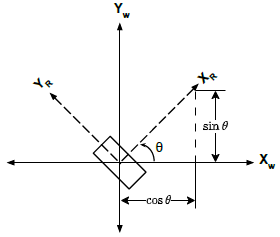
\includegraphics[width=0.45\textwidth]{q9.png}}
%				\captionof{figure}{World coordinate system and Robot coordinate system}
%				\label{fig:q9}
%				\vspace{0.5cm}
%			\end{minipage}
%			And the standard basis for the world frame, 
%			\begin{equation} {[x]}_{W} = 
%				\left(
%					{X}_{W} = \begin{bmatrix}1 \\ 0\end{bmatrix},
%					{Y}_{W} = \begin{bmatrix}0 \\ 1\end{bmatrix}
%				\right)
%			\end{equation}
%			
%			It is given that the rotated by an angle $\theta$ as shown in Figure ~\ref{fig:q9}. 
%			
%			So, we get the new basis by applying trogonometric relations as, 
%			\begin{equation} {[x]}_{R} = 
%				\left(
%					{X}_{R} = \begin{bmatrix}\cos\theta \\ \sin\theta\end{bmatrix},
%					{Y}_{R} = \begin{bmatrix}-\sin\theta \\ \cos\theta\end{bmatrix}
%				\right)
%			\end{equation}
%			
%			Now, we need to find a matrix $P$ such that,  ${[x]}_{R} = P{[x]}_{W}$
%			
%			But as it is easier to find $\bar{P}$ first, we shall do it by working column by column, 
%			\renewcommand{\arraystretch}{1.5}
%			\begin{equation}\bar{P} = \left[\begin{array}{c:c} {\bar{P}}_{1} &  {\bar{P}}_{2}\end{array}\right]\end{equation}
%			
%			\begin{equation}{\bar{P}}_{1} = {[{X}_{R}]}_{W} = \begin{bmatrix}\cos\theta \\ \sin\theta\end{bmatrix} \;
%			{\bar{P}}_{2} = {[{Y}_{R}]}_{W} = \begin{bmatrix}-\sin\theta \\ \cos\theta\end{bmatrix}
%			\Rightarrow \bar{P} = \begin{bmatrix} \cos\theta & -\sin\theta \\ \sin\theta & \cos\theta\end{bmatrix}\end{equation}
%			
%			As, $\bar{P} = {P}^{-1}$ $\Rightarrow P = {\bar{P}}^{-1}, $ 
%			\begin{equation}
%				\Rightarrow P = \frac{1}{{\cos}^{2}\theta + {\sin}^{2}\theta}\begin{bmatrix}\cos\theta & \sin\theta \\-\sin\theta & \cos\theta\end{bmatrix}
%			\end{equation}
%			
%			\begin{equation}
%				=\begin{bmatrix}\cos\theta & \sin\theta \\-\sin\theta & \cos\theta\end{bmatrix}
%			\end{equation}
%			
%		
%%		\item[Question: 10. (a) ] \setcounter{equation}{0} %Nagy, Page 136, Prob. 4.4.4 (a)
%%		\item[Answer:] Given,
%%			$\mathcal{M} = ({M}_{1}, {M}_{2}, {M}_{3}, {M}_{4}) \subset {\mathbb{R}}^{2,2}$ with, \\ \\
%%			${M}_{1} = \begin{bmatrix}0 & 1 \\ 1 & 0\end{bmatrix}$,	${M}_{2} = \begin{bmatrix}0 & -1 \\ 1 & 0\end{bmatrix}$,	${M}_{3} = \begin{bmatrix}1 & 0 \\ 0 & 1\end{bmatrix}$,	${M}_{4} = \begin{bmatrix}1 & 0 \\ 0 & -1\end{bmatrix}$ 
%%			
%%			Firstly, we shall check for the \textit{Linear Independence} of $\mathcal{M}$
%%			\begin{equation}
%%				\Rightarrow {\alpha}_{1}\begin{bmatrix}0 & 1 \\ 1 & 0\end{bmatrix} + {\alpha}_{2}\begin{bmatrix}0 & -1 \\ 1 & 0\end{bmatrix} + {\alpha}_{3}\begin{bmatrix}1 & 0 \\ 0 & 1\end{bmatrix} + {\alpha}_{4}\begin{bmatrix}1 & 0 \\ 0 & -1\end{bmatrix} = 0
%%			\end{equation}
%%			\begin{align}
%%				\Rightarrow {\alpha}_{3} + {\alpha}_{4} = 0 \\
%%				\Rightarrow {\alpha}_{1} - {\alpha}_{2} = 0 \\
%%				\Rightarrow {\alpha}_{1} + {\alpha}_{2} = 0 \\
%%				\Rightarrow {\alpha}_{3} - {\alpha}_{4} = 0
%%			\end{align}
%%			Upon solving ${Eq}^{n} (2), (3), (4), (5), $ we get, ${\alpha}_{1} = {\alpha}_{2} = {\alpha}_{3} = {\alpha}_{4} = 0.$
%%			
%%			$\Rightarrow \; \mathcal{M}$ is \textit{Linearly Independent}. \\ \\
%%			
%%			Secondly, $span\{\mathcal{M}\} = {\mathbb{R}}^{2,2}$ 
%%			
%%			Consider some arbitraty matrix, 
%%			\begin{equation}R = \begin{bmatrix}{r}_{11} & {r}_{12} \\ {r}_{21} & {r}_{22} \end{bmatrix} \subset {\mathbb{R}}^{2,2}\end{equation}
%%			
%%			Now, let us try to express $R$ as a linear combination of $\mathcal{M}$, 
%%			\begin{equation}
%%				R = {\beta}_{1}{M}_{1} + {\beta}_{2}{M}_{2} + {\beta}_{3}{M}_{3} + {\beta}_{4}{M}_{4}
%%			\end{equation}
%%			\begin{equation}
%%				\begin{bmatrix}{r}_{11} & {r}_{12} \\ {r}_{21} & {r}_{22} \end{bmatrix} = {\beta}_{1}\begin{bmatrix}0 & 1 \\ 1 & 0\end{bmatrix} + {\beta}_{2}\begin{bmatrix}0 & -1 \\ 1 & 0\end{bmatrix} + {\beta}_{3}\begin{bmatrix}1 & 0 \\ 0 & 1\end{bmatrix} + {\beta}_{4}\begin{bmatrix}1 & 0 \\ 0 & -1\end{bmatrix}
%%			\end{equation}
%%			\begin{align}
%%				\Rightarrow {r}_{11} = {\beta}_{3} + {\beta}_{4} \\
%%				\Rightarrow {r}_{12} = {\beta}_{1} - {\beta}_{2} \\
%%				\Rightarrow {r}_{21} = {\beta}_{1} + {\beta}_{2} \\
%%				\Rightarrow {r}_{22} = {\beta}_{3} - {\beta}_{4}
%%			\end{align}
%%			Where, ${r}_{11}, {r}_{12}, {r}_{21}, {r}_{22}, {\beta}_{1}, {\beta}_{2}, {\beta}_{3}\; and\; {\beta}_{4} \in \mathbb{R} $ \\
%%			Since we have expressed an arbitrary matrix $R$ as a linear combination of the matrices in $\mathcal{M}$ with coefficients that can be any real values, this means that $\text{span}\{\mathcal{M}\}$ can generate any matrix in $\mathbb{R}^{2,2}$. \\
%%			$\Rightarrow\text{span}\{\mathcal{M}\} = \mathbb{R}^{2,2}$
%%			
%%			Having proved that $\mathcal{M}$ is both \textit{Linearly Independent} and $\text{span}\{\mathcal{M}\} = \mathbb{R}^{2,2}$ \\
%%			$\therefore$ the set $\mathcal{M}$ is a basis of ${\mathbb{R}}^{2,2}$. \textbf{Q.E.D}
%%						
%%		\item[Question: 10. (b) ] \setcounter{equation}{0} %Nagy, Page 136, Prob. 4.4.4 (b)
%%		\item[Answer:] Given,
%%			\begin{equation}
%%				A = \begin{bmatrix}1 & 2 \\ 3 & 4\end{bmatrix}
%%			\end{equation}
%%			And $\mathcal{M} = ({M}_{1}, {M}_{2}, {M}_{3}, {M}_{4}) \subset  \mathbb{R}^{2,2}$ with, \\ \\
%%			${M}_{1} = \begin{bmatrix}0 & 1 \\ 1 & 0\end{bmatrix}$,	${M}_{2} = \begin{bmatrix}0 & -1 \\ 1 & 0\end{bmatrix}$,	${M}_{3} = \begin{bmatrix}1 & 0 \\ 0 & 1\end{bmatrix}$,	${M}_{4} = \begin{bmatrix}1 & 0 \\ 0 & -1\end{bmatrix}$ 
%%			To find the components of $A$ in the ordered basis $\mathcal{M}$, we must put it in the form of a linear combination, 
%%			\begin{equation}
%%				{\alpha}_{1}{M}_{1} + {\alpha}_{2}{M}_{2} + {\alpha}_{3}{M}_{3} + {\alpha}_{4}{M}_{4} = A
%%			\end{equation}
%%			\begin{equation}
%%				{\alpha}_{1}\begin{bmatrix}0 & 1 \\ 1 & 0\end{bmatrix} + {\alpha}_{2}\begin{bmatrix}0 & -1 \\ 1 & 0\end{bmatrix} + {\alpha}_{3}\begin{bmatrix}1 & 0 \\ 0 & 1\end{bmatrix} + {\alpha}_{4} \begin{bmatrix}1 & 0 \\ 0 & -1\end{bmatrix} = \begin{bmatrix}1 & 2 \\ 3 & 4\end{bmatrix}
%%			\end{equation}
%%			\begin{align}
%%				\Rightarrow {\alpha}_{3} + {\alpha}_{4} = 1 \\
%%				\Rightarrow {\alpha}_{1} - {\alpha}_{2} = 2\\
%%				\Rightarrow {\alpha}_{1} + {\alpha}_{2} = 3 \\
%%				\Rightarrow {\alpha}_{3} - {\alpha}_{4} = 4
%%			\end{align}
%%			Upon solving ${Eq}^{n} (4), (5), (6), (7), $ we get, ${\alpha}_{1} = \frac{5}{2}$ ; ${\alpha}_{2} = \frac{1}{2}$ ; ${\alpha}_{3} = \frac{5}{2}$ ; ${\alpha}_{4} = -\frac{3}{2}$
%%			Therefore, 
%%			\begin{equation} \notag
%%				\begin{bmatrix}1 & 2 \\ 3 & 4\end{bmatrix}= \frac{5}{2}{M}_{1} + \frac{1}{2}{M}_{2} + \frac{5}{2}{M}_{3} - \frac{3}{2}{M}_{4} \iff {[A]}_{\mathcal{M}} = \begin{bmatrix}\frac{5}{2} & \frac{1}{2} \\ \frac{5}{2} & -\frac{3}{2}\end{bmatrix} \in {\mathbb{R}}^{2,2}
%%			\end{equation}
	\end{qalist}
\end{document}